\documentclass[letterpaper, 12pt]{article}
\usepackage[spanish]{babel}
\usepackage{graphicx}
\usepackage{multicol}
\usepackage{anysize}
\usepackage{fontspec}
\usepackage{lineno}
\usepackage{lipsum}
\usepackage{listings}
\usepackage{verbatim}
\usepackage{python}
\usepackage{amsmath}
\graphicspath{/home/mohammed/Desktop/APlab/Week2}
\setlength\columnsep{30pt} %Espacio entre columnas
\renewcommand{\familydefault}{\sfdefault}

% MÁRGENES
\marginsize{30pt}%izquierda
{30pt} %derecha
{10pt} %arriba
{20pt} %abajo
%


\begin{document}
\begin{center}
\Huge Assignment-2 
\vspace{3mm}
\rule[0mm]{20mm}{0.2mm}
\vspace{-8mm}
\begin{multicols}{2}
\begin{flushleft}
\begin{large}
\texttt{EE2703-Applied Programming Lab}\\
\end{large}
\end{flushleft}
\begin{flushright}
\begin{small}
\texttt{1 Feb 2018}
\end{small}
\end{flushright}
\end{multicols}
\vspace{5mm}
\end{center}
\vspace{-14mm}
\begin{center}
\begin{huge}
\textbf{Vector Operations and Functions in Python}
\end{huge}
\end{center}
\vspace{2mm}
\rule[10mm]{20mm}{0.5mm}
\begin{multicols}{2}
\begin{flushleft}
\begin{Large}
\textbf{Mohammed Khandwawala}
\end{Large}
\end{flushleft}
\begin{flushright}
\textbf{EE16B117}
\end{flushright}
\end{multicols}
\tableofcontents
\clearpage
\begin{multicols}{2}
\section{Introduction}
Python is the most commonly used tool for scientic computing, engineering, and research.
It is comparable with well-established softwares like MATLAB and even better in some aspects. A major cause is its open-source nature and huge base of python contributor. This is the reason why python tends to be very quick at incorporating
useful features from other languages.
Python is best among other programming languages in string manipulation. 
Some useful python scientific packages include scipy , numpy and matplotlib. These packages are taken together an bundled in pylab module which has all kind of matlab functionality.
This assignment introduces vector operations provided by
numpy and the calculation of definite integrals using the quad function.
\subsection{Numpy arrays for vector operation}
Numpy module in python consist of important numerical functions. One of the feature it has is numpy arrays which are much easier to use than C arrays and hence can handle much complex tasks. Numpy arrays are better for numerically extensive jobs than native lists.
\subsection{Scipy : The Library for Scientific Computations}
Scipy is an extensive package containing functions for scientific uses. In this assignment we are using quad function from scipy.integrate to calculate integral. 
\subsection{Matplotlib : The Plotting Library}
It is a very powerful plotting package. It allows to plot various type of multidimensional plots , of various types and offer great amount of customizations on how the plot looks unlike MATLAB. 
\section{Function Defination}
The function defined is a general python function and like all python function returns a vector if a vector is passed to it.
\vspace{6mm}
\begin{footnotesize}
\textit{Format: x = arange([start,] stop[, step], dtype = None)}
\end{footnotesize}
Above line shows the format for generating vectors.
plt.title adds the title to the plot and plt.scatter plots the scatter plot between first and second argument passed to the function.
\begin{lstlisting}[language=Python ,caption=To generate and plot $1/(1+t^{2})$]
import matplotlib.pyplot as plt
import numpy as np
import math

def taninf(x):
	return 1/(1+x**2)

x = np.arange(0,5.1,0.1)

val = taninf(x)

plt.scatter(x,val)
plt.title(r"Plot of $1/(1+t^{2})$")
plt.show()
\end{lstlisting}
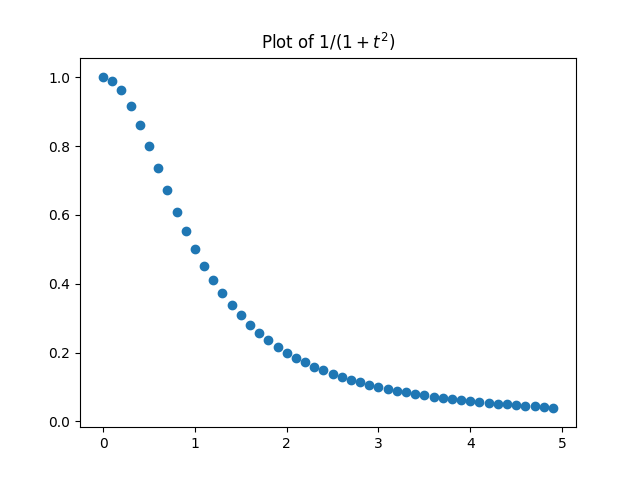
\includegraphics[width=\columnwidth]{Figure_1.png}
\section{Integration Using quad function}
To compute integral using quad function function definition and the limits are need to be passed. The function returns two values for a point. First value is the value of the integral and second is the error.
\begin{lstlisting}[language=Python , caption=Using quad function to integrate $1/(1+t^{2})$]
from scipy.integrate import quad
integration = []

for i in range(0,len(x)):
	temp = quad(taninf,0,x[i])
	integration.append(temp[0])

plt.scatter(x,val,c='red')
plt.plot(x,integration,c="black")
plt.legend(("quadfn",r"Plot of ...
...$1/(1+t^{2})$"))
plt.show()
\end{lstlisting}
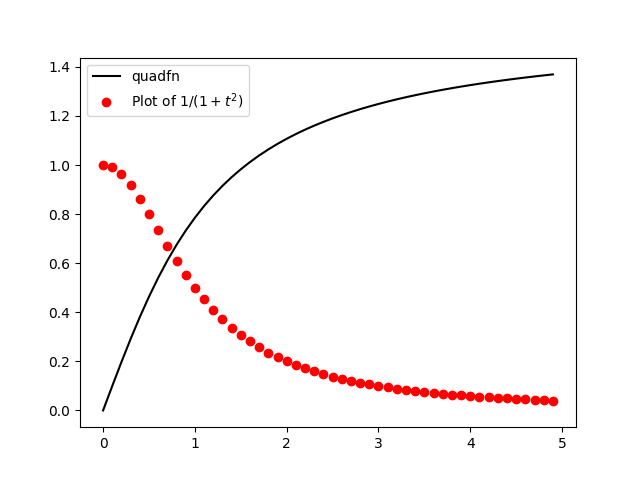
\includegraphics[width=\columnwidth]{Figure_1-1.png}
\subsection{Tabulated Values of quad function integral values of $1/(1+t^{2})$ values against x}
To tabulate the result built in python function tabulate can be used. It accepts table , 2-D array of data-frame. So to tabulate arctan(x) with quad function using pandas their respaective array is converted into data-frame which is than tabulated.  
\begin{lstlisting}[language=Python , caption=Tabulating Quad function integral of $1/(1+t^{2})$ against x]
import pandas as pd
from tabulate import tabulate

table = pd.DataFrame({"x":x,"Quad...
...Function Integral":integration})
print tabulate(table, headers=...
...'keys',tablefmt='p')
\end{lstlisting}
\end{multicols}
\begin{flushleft}
\verbatiminput{out.txt}
\end{flushleft}
\begin{multicols}{2}
\begin{lstlisting} [float=h,frame=tb,caption=R output,label=zebra]{out.txt}
\end{lstlisting}
\section{Comparing Quad function integral with actual value of tan$^{-1}$(x)}
Plotting both actual value and the integral value via quad function show the accuracy of computation. Plots closely resemble.
\begin{lstlisting}[language=Python , caption=Comparing Quad function integal with actual value of tan$^{-1}$(x)]

atan = np.arctan(x)

plt.scatter(x,integration,c='red')
plt.plot(x,atan,c="black")
plt.legend(("quadfunction",...
...r"tan$^{-1}$(x)"))
plt.show()
\end{lstlisting}
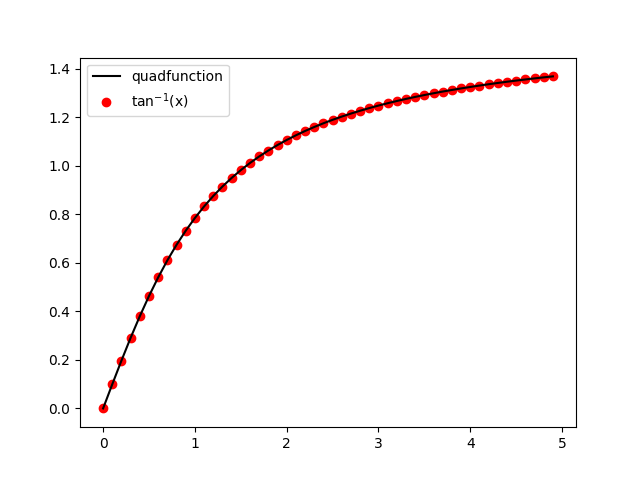
\includegraphics[width=\columnwidth]{Figure_1-2.png}
\section{Computing difference between Quad function integal with actual value of tan$^{-1}$(x)}
The difference plot between the both clearly shows the deviation in the range of 10$^{-15}$.
\end{multicols}
\begin{lstlisting}[language=Python , caption=Comparing Quad function integal with actual value of tan$^{-1}$(x)]
integration = np.array(integration)
error = abs(integration - atan)

plt.semilogy(x,error,"ro")
plt.title("Error between quad function and tan$^{-1}$(x) value")	
plt.show()
\end{lstlisting}
\begin{multicols}{2}
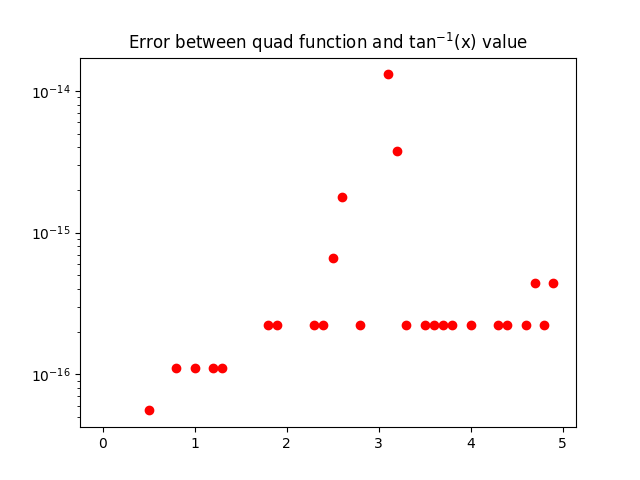
\includegraphics[width=\columnwidth]{Figure_1-3.png}
\section{Integration using trapezoidal algorithm }
\subsection{About}
According to the Trapezoidal Rule, if a function is known at points a, a + h,..., b, its integral is
given by
\begin{center}
	\[ \begin{cases} 
      0 & x = 0 \\
      0.5( \textit{f(a) + f(x$_{i}$}) +  $$\sum_{j=1}^{i-1}\textit{f(x$_{j}$)} $$ &  x = a + ih \\
   \end{cases}
\]
\end{center}
or it can be rearranged as
\begin{center}
\vspace{1mm}
	\textit{I$_{i}$}=\textit{h ( $\sum_{j=1}^{i}\textit{f(x$_{j}$) - $\frac{1}{2}$ ( f(x$_{j}$) + f(x$_{j}$) )}$} )
\vspace{1mm}
\end{center}
The last equation can simply be computer in one line using cumsum() function which calculates the cumulative sum for every index of vector.
\subsection{Computing trapezoidal Integral using a loop}
Using the above defined formula trapezoidal integral can easily computed in a for loop.
\end{multicols}
\begin{lstlisting}
def trapz(a,b,h):
    y=np.zeros(int((b-a)/h)+1)
    
    for i in range(1,len(y)):
        y[i]=y[i-1]+0.5*h*(taninf(a+i*h)+taninf(a+(i-1)*h))
    return y
\end{lstlisting}
\begin{multicols}{2}
\subsection{Computing trapezoidal Integral by passing vector as argument}
Code below shows a much simpler way of computing trapezoidal integral from the same formula using vectors. This implementation does not require to write a for loop.
\end{multicols}
\begin{lstlisting}[language=Python , caption=Comparing Quad function integal with actual value of tan$^{-1}$(x)]
h=0.1
n=5/h

pts = np.arange(0,5,h)
tanval = taninf(pts)
c_sum = np.cumsum(tanval)
trapz = h*(c_sum-(tanval[0]+tanval)/2)
plt.scatter(pts,trapz)
plt.title(r"Plot of $\int_{0}^{5}$ ...
...$1/(1+t^{2})$ dx using trapz")
plt.show()
\end{lstlisting}
\begin{multicols}{2}
\section{Computing Error}
\subsection{Exact Error}
Exact error is ( for a fixed h) computed by taking the maximum of the absolute difference between the value of tan$^{-1}$(x) and integral value by trapezoidal function at each x.
\subsection{Estimated Error}
Estimated error is calculates by taking the maximum value of absolute difference between the integral values ( generated by trapezoidal function ) between consecutive iteration of reduced step size (h) at common points . Here in this case starting value of step-size is 0.5 and reduced by half in every iteration. Error computing loop in iterated 12 times to get desired tolerance of 10${-8}$.
\end{multicols}
\begin{lstlisting}[language=Python , caption=Computing estimated and exact error and plotting them.]
H = []
estimated_error = []
exact_error = []

h=1
pts = np.arange(0,5,h)
tanval = taninf(pts)
c_sum = np.cumsum(tanval)
trapz = h*(c_sum-(tanval[0]+tanval)/2)
h = 0.5
for i in range(12):
	pts_2 = np.arange(0,5,h)
	tanval_2 = taninf(pts_2)
	act_val = np.arctan(pts_2)
	c_sum_2 = np.cumsum(tanval_2)
	trapz_2 = h*(c_sum_2-(tanval_2[0]+tanval_2)/2)	
	if(i!=0):
		es_err = abs(trapz - trapz_2[::2])
		estimated_error.append(max(es_err))
	ex_err = abs(trapz_2 - act_val)
	exact_error.append(max(ex_err))
	H.append(h)
	trapz = np.array(trapz_2)
	h=h/2
plt.loglog(H[1:],estimated_error,"g+")
plt.loglog(H,exact_error,"ro")
plt.legend(("Estimated Error","Exact Error"))
plt.show()
\end{lstlisting}
\begin{multicols}{2}
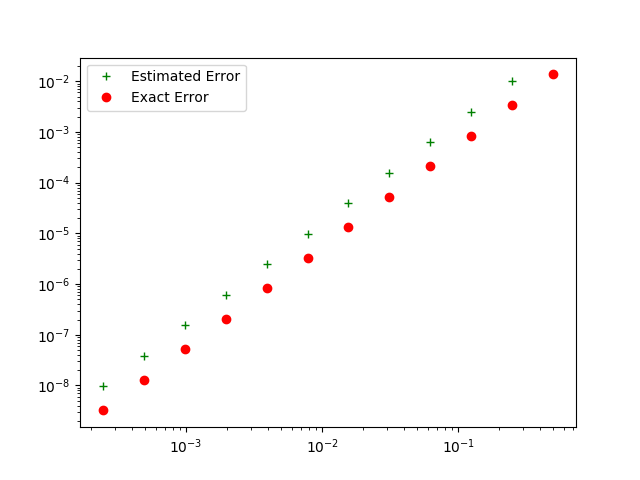
\includegraphics[width=\columnwidth]{Figure_1-5.png}
\section{Conclusion}
The python implementation of MATLAB like libraries i.e. scipy, numpy and matplotlib and accurate and powerful.Adopted matlab functions are improved in functionality in pythons implementation.   
\begin{flushright}
\end{flushright}
\end{multicols}
\end{document}

